% ----------------------------------------------------------------------

\chapter{\textbf{Referencial Teórico}}

Nesse capítulo são apresentados os principais conceitos referentes às técnicas aplicadas no desenvolvimento do trabalho, referenciando a literatura e autores utilizados para explicação dos respectivos temas.

\section{Sistemas de Recomendação}

O sistema de recomendação é definido como uma estratégia de tomada de decisão para usuários em ambientes de informação complexos \cite{rashid2002}. Desse modo, a utilização de sistemas de recomendação permite que o usuário consiga lidar com grandes quantidades de informação, provendo recomendações personalizadas e exclusivas do conteúdo analisado \cite{isinkaye2015}.

Para desenvolvimento de um sistema de recomendação, diversos fatores devem ser levados em consideração. De acordo com \citeonline{kimfalk2019}, os seguintes componentes podem ser definidos como a taxonomia \footnote{Taxonomia: no caso citado refere-se a estrutura básica de um sistema de recomendação} de um sistema de recomendação:

\begin{itemize}
	\item \textbf{Domínio}: Refere-se ao tipo de conteúdo recomendado. Com base nesse dado é possível entender, com mais facilidade, o que fazer com as recomendações geradas. Ademais, o conhecimento do domínio possibilita saber qual o custo e impacto que uma recomendação errada poderá gerar ao sistema.
	
	\item \textbf{Objetivo}: Define qual será o foco e estratégia utilizado em cima da recomendação gerada. Principalmente no meio comercial, recomendações com certa tendência a algum produto ou serviço específico podem gerar mais benefícios e lucros para seus criadores, fazendo com que o objetivo da recomendação gere um impacto direto no sistema desenvolvido.
	
	\item \textbf{Contexto}: Refere-se ao ambiente no qual o consumidor utilizará o sistema de recomendação. Esse dado é importante, uma vez que possibilita definir qual será a melhor tecnologia e técnica utilizada no sistema de recomendação. 
	
	\item \textbf{Níveis de personalização}: As recomendações podem apresentar diversos níveis de personalização para seu usuário final, sendo que essas personalizações podem ser divididas em três níveis:
	
	\begin{itemize}
		\item \textit{Não-personalizada}: apresenta as recomendações de forma padronizada para todos os usuários do sistema. Como exemplos típicos dessa abordagem pode-se citar a lista de itens mais populares em um sistema voltado para comércio.
		
		\item \textit{Semi-personalizada ou dividida em segmento}: nesse modelo, o sistema de recomendação procura agrupar os usuários de forma a gerar recomendações voltadas aos interesses de cada grupo.
		
		\item \textit{Personalizada}: nesta abordagem o sistema busca realizar recomendações de acordo com interações passadas do usuário, gerando resultados exclusivos para cada um deles.
	\end{itemize}

	\item \textbf{Quem recomenda}: Em casos específicos, a opinião de especialistas pode apresentar relevância no momento da construção da recomendação, nestes casos, é necessário que esse item seja levado em consideração no desenvolvimento do sistema.
	
	\item \textbf{Privacidade e confiabilidade}: A forma como lidamos com os dados informados e gerados dos usuários é outra questão bastante relevante a ser analisada nos sistemas de recomendação, principalmente em contextos onde informações sigilosas e sensíveis são manipuladas. A confiabilidade refere-se ao quanto o usuário confia nas recomendações ao invés de considerá-las como propagandas ou tentativas de manipulação. O sistema é mais confiável de acordo com que o usuário aceita as recomendações seriamente.
	
	\item \textbf{Interface}: Refere-se aos métodos utilizados para comunicar o usuário ao sistema de recomendação, sendo dividido em \textit{input}: entrada de dados do usuário (de forma explícita ou implícita) e \textit{output}: retorno da recomendação pelo sistema. Em relação ao \textit{output}, pode ser interessante em alguns casos explicar ao usuário como a recomendação é feita. Em um dos estudos de \citeonline{kimfalk2019}, demonstrado na figura \ref{fig:explicabilidade}, é possível analisar a relação entre o nível de acurácia da recomendação e a facilidade de explicação ao usuário de como a mesma foi feita:
	
	\begin{figure}[H]
		\centering
		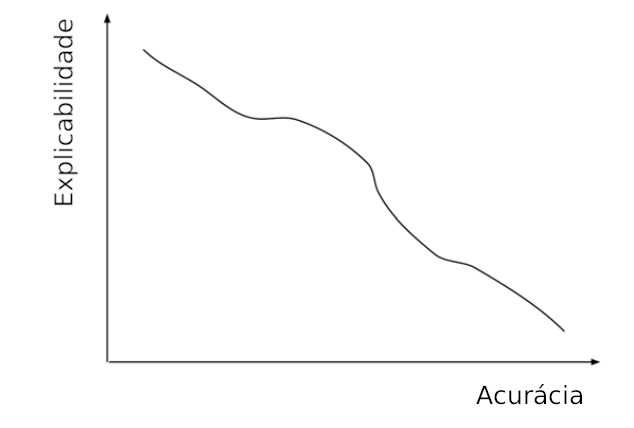
\includegraphics[width=0.7\linewidth]{imagens/explicabilidade}
		\caption[Explicabildade vs. qualidade da recomendação]{Explicabildade vs. qualidade da recomendação}
		\label{fig:explicabilidade}
	\end{figure}
	 
	\item \textbf{Algoritmos}: Existem diversos algoritmos que podem ser utilizados na construção de um sistema de recomendação. Esses algoritmos costumam ser divididos em dois grupos: \textbf{filtragem colaborativa} e \textbf{baseada em conteúdo}, sendo que a escolha do tipo de algoritmo dependerá do tipo de dado utilizado para construção das recomendações. Uma abordagem \textbf{híbrida} também pode ser utilizada, mesclando técnicas dos dois grupos apresentados.
\end{itemize}

\subsection{Filtragem Colaborativa}

O algoritmos de filtragem colaborativa têm como objetivo explorar informações a partir das experiências dos usuários para recomendação de itens \cite{sedhain2015}. Para isso, esses algoritmos utilizam técnicas como a fatoração matricial como apresentado por \citeonline{koren2009}, \citeonline{lee2013} e modelos de vizinhança como definido por \citeonline{sarwar2001}, de forma a recomendar itens parecidos para usuários com certo nível de proximidade \cite{kimfalk2019}.

Um dos problemas ao utilizar-se dessa abordagem é a dependência existente entre a recomendação e os dados dos demais usuários, fazendo com que as recomendações geradas na fase inicial desses sistemas possam apresentar desvios nos resultados gerados \citeonline{wei2017collaborative} e \cite{choi2010content}.

Esse modelo de recomendação é bastante conhecido, sendo um dos mais utilizados nos sistemas de recomendação \cite{alyari2018}.

\subsection{Filtragem baseada em Conteúdo}

A filtragem baseada em conteúdo, como definido por \citeonline{kimfalk2019}, é um modelo de algoritmo que utiliza de metadados para gerar as recomendações dos itens. Nesses sistemas, é buscada a criação de um perfil para os usuários baseado nos itens do sistema, de forma com que seja possível comparar esse perfil aos itens para geração das recomendações.

Como principal problema dessa abordagem de recomendação têm-se o momento em que um novo usuário acaba de ser criado, uma vez que o sistema não consegue inferir quais são os tópicos (assuntos ou tags) de maior relevância para esse usuário, reduzindo a taxa de acertos nas recomendações iniciais \cite{inbook}.

\subsection{Recomendação Híbrida}

Abordagens de recomendação colaborativas e baseadas em conteúdo apresentam pontos positivos e negativos \cite{kimfalk2019}. A recomendação baseada em conteúdo apresenta alguns problemas associados a análise limitada das informações, superespecialização e escassez de dados como demonstrado por \citeonline{adomavicius2005}, enquanto que a abordagem colaborativa apresenta problemas relacionados principalmente a escalabilidade e manipulação de bases com baixo volume de dados \cite{isinkaye2015}.

Com intuito de melhorar a qualidade da recomendação e como forma de mitigar alguns dos problemas identificados, foi proposto o modelo de filtragem híbrida, que busca a partir da combinação das técnicas de filtragem, aumentar o desempenho e precisão dos sistemas de recomendação \cite{goksedef2010}. Com essa abordagem, busca-se aproveitar os pontos fortes vistos em cada uma das abordagens, como também, nivelar suas fraquezas \cite{al2008}. 

Diversas estratégias podem ser utilizadas na recomendação híbrida, onde as principais, levando em conta a forma como os componentes serão combinados para gerar as recomendações, são as seguintes  \cite{barbosa2014}:

\begin{itemize}
    \item \textbf{Ponderada:} nesse modelo de abordagem, as filtragens colaborativa e baseada em conteúdo são aplicadas de forma separada, sendo que, após a geração das recomendações, é realizado um processo de combinação linear, utilizando os resultados gerados. Em alguns casos, pode ser necessário a realização de uma normalização entre os dados, caso os mesmos estejam em escalas diferentes.
    
    \item \textbf{Mista:} nesse modelo as recomendações geradas são mescladas para geração do resultado final. Desde modo, o resultado apresentado ao usuário será uma lista com os dados gerados na recomendação colaborativa e baseada em conteúdo.
    
    \item \textbf{Combinação sequencial:} nesse modelo temos a criação de um perfil do usuário, em um primeiro momento, a partir da recomendação baseada em conteúdo. A partir dos perfis criados, é realizada a recomendação colaborativa que gerará os resultados finais dessa abordagem.
    
    \item \textbf{Comutação:} para essa abordagem, é necessário a utilização de algum critério para avaliação, que pode ser definido de acordo com a natureza do sistema. Esse critério é utilizado para comutar ou chavear os resultados obtidos na recomendação colaborativa e baseada em conteúdo, gerando o resultado final. Outra abordagem válida é a comutação de uma técnica nos pontos de desvantagens da outra.
\end{itemize}

Vale ressaltar, que a escolha da metodologia aplicada variará de acordo com a natureza do problema em questão.

\subsection{Matriz de Recomendação offline}

O processo de recomendação nos sistemas, pode ocorrer de três maneiras diferentes: recomendação online, offline e a combinação das duas formas anteriores. De acordo com \citeonline{gunawardana2009survey} a recomendação offline deve ser utilizada para identificação dos itens mais promissores, para que os mesmos possam ser submetidos ao processo de recomendação online.

Para realização dessa abordagem, é necessário o armazenamento do conjunto de dados utilizados na recomendação, sendo que, segundo \citeonline{gunawardana2009survey}, os dados devem se assemelhar o máximo possível com os dados usados na abordagem online. Utilizando essa técnica de recomendação têm-se uma melhoria na performance do processo, uma vez que se diminui o tempo da tarefa de recomendação no ponto de vista dos utilizadores \cite{moreira2019sistema}.

\section{Programação Concorrente}

Em diversas aplicações, múltiplas atividades podem ocorrer ao mesmo tempo. Desse modo, é possível decompor uma aplicação em múltiplas threads(linhas de execução) sequenciais que executem de forma paralela \cite{tanenbaum2015modern}. Pode-se analisar, na figura \ref{fig:threads}, um exemplo de sistema de edição de texto utilizando três threads simultaneamente. Nesse exemplo simplificado, é possível observar as seguintes funções para cada thread:

\begin{itemize}
    \item \textbf{Thread 1:} Receber os dados informados pelo teclado;
    \item \textbf{Thread 2:} Exibir o texto no editor (tela da aplicação);
    \item \textbf{Thread 3:} Salvar os dados informados no disco (função de auto-salvamento).
\end{itemize}

\begin{figure}[H]
		\centering
		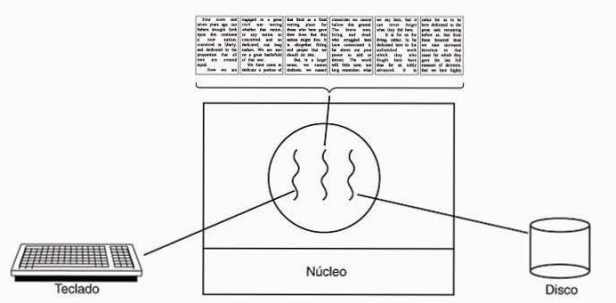
\includegraphics[width=0.8\linewidth]{imagens/threads.png}
		\caption[Uso de threads em um sistema de edição de texto]{Uso de threads em um sistema de edição de texto \cite{tanenbaum2007distributed}}
		\label{fig:threads}
	\end{figure}

O uso de threads possibilita o aumento de desempenho das aplicações que possuem muitos processos de E/S, devido a sobreposição possível entre as linhas de execução \cite{tanenbaum2015modern}.

\textbf{Diferença entre threads e processos}

Segundo \citeonline{tanenbaum2015modern}, um processo pode ser definido como um programa em execução que possui valores de um contador de programa (que define até onde o processo já foi executado), registradores e variáveis. Desse modo, os processos podem ser considerados programas independentes, sendo executados de acordo com o escalonamento definido pelo sistema operacional. Na figura \ref{fig:processos}, é possível visualizar uma exemplo de execução de quatro processos em um sistema:

\begin{figure}[H]
		\centering
		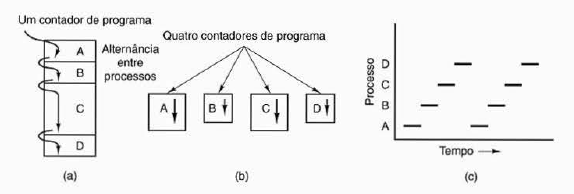
\includegraphics[width=1\linewidth]{imagens/processos.png}
		\caption[Exemplo de execução de quatro processos]{Exemplo de execução de quatro processos \cite{tanenbaum2015modern}}
		\label{fig:processos}
	\end{figure}

Enquanto isso, uma thread pode ser considerada uma linha de execução que compartilha recursos e o espaço de endereçamento da memória, executando de forma quase paralela \cite{tanenbaum2015modern}. A principal razão para seu uso é em aplicações onde ocorram diversas operações ao mesmo tempo, fazendo com que o modelo de programação seja facilitado a partir do uso de threads \cite{tanenbaum2015modern}.

Como definido por \citeonline{tanenbaum2015modern}, existe três argumentos para utilização de threads em um sistema:

\begin{itemize}
    \item \textbf{Compartilhamento de recursos:} capacidade de entidades paralelas compartilharem um mesmo espaço de endereçamento de memória e dados.
    \item \textbf{Velocidade:} as threads são mais fáceis e rápidas de serem destruídas que os processos, uma vez que não possuem quaisquer recursos vinculados a elas. Além disso, em muitos sistemas, a criação de threads é cerca de até cem vezes mais rápida que a criação de um processo. Esse fator é bastante útil em aplicações que o número de threads se altera de forma rápida e dinâmica.
    \item \textbf{Desempenho:} a utilização de threads em processos de E/S (entrada e saída) pode resultar em melhoria de performance da aplicação, já que as threads possibilitam a sobreposição dessas tarefas. 
\end{itemize}

\subsection{Ciclos de Vida e estados da thread}

Durante a execução de um programa concorrente, uma thread pode apresentar vários estados, como definido por \citeonline{deitel2016} e apresentado na figura \ref{fig:ciclovidathread}:

\begin{figure}[H]
	\centering
	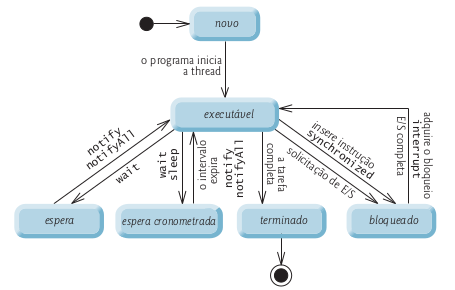
\includegraphics[width=0.8\linewidth]{imagens/cicloVidaThread}
	\caption[Estado e ciclo de vida da thread]{Diagrama de estado e ciclo de vida da thread \cite{deitel2016}}
	\label{fig:ciclovidathread}
\end{figure}

Muitos desses estados são abstraídos pelas linguagens de programação de alto nível, simplificando o processo de desenvolvimento. Porém, para aplicações com rotinas mais avançadas, o conhecimento desses estados e o ciclo de vida das threads torna-se trivial, pois permite ao programador um maior nível de controle sobre o software \cite{deitel2016}. Dessa forma, baseando na obra de \citeonline{deitel2016}, é apresentado abaixo os ciclos e estados que uma thread pode obter durante a execução de um software concorrente.

\textbf{Estado novo e executável}

Uma nova thread tem seu ciclo de vida iniciado com o estado \textbf{novo}. Esse estado é mantido até que o programa inicie a thread, mudando seu estado para \textbf{executável}, que é mantido enquanto essa thread encontra-se em execução.

\textbf{Estado de espera}

Uma thread em estado \textit{executável} transita para o estado de \textbf{espera} quando é necessário aguardar que outra thread realize alguma tarefa. A thread em \textit{espera} volta ao estado \textit{executável} quando é notificada por outra thread que continue sua execução.

\textbf{Estado de espera sincronizada}

Uma thread que está no estado \textit{executável} pode entrar no estado de \textbf{espera sincronizada} por um determinado período de tempo, voltando para o estado \textit{executável} após término desse período ou de um evento que ela esteja aguardando. Threads nesse estado não poderão utilizar o processador, mesmo que ele esteja disponível.

Em determinadas situações, uma thread \textit{executável} pode transitar para o estado de \textit{espera sincronizada} ao fornecer um intervalo de espera opcional, procurando, dessa forma, esperar a realização de alguma tarefa realizada por outra thread.

\textbf{Estado bloqueado}

Uma thread \textit{executável} pode entrar no estado \textbf{bloqueado} ao tentar realizar uma tarefa que não pode ser concluída imediatamente, fazendo com que a thread tenha que esperar até que a tarefa bloqueante seja concluída. Threads nesse estado não poderão acessar o processador, mesmo que ele esteja disponível.

\textbf{Estado terminado}

Ocorre quando uma thread \textit{executável} conclui com sucesso sua tarefa, o que faz com que a mesma mude para o estado \textbf{terminado} (às vezes chamado de estado \textbf{morto}). Esse estado também pode ocorrer caso a thread seja terminada por outro motivo, como razão de um erro, por exemplo. 

\subsection{Sincronização de threads}

Em momentos que várias threads compartilham um objeto que é modificado por uma ou mais delas, podem ocorrer resultados indeterminados caso a manipulação e acesso a esse objeto ocorra de forma incorreta. Neste tipo de caso, o comportamento do programa torna-se não confiável, uma vez que os resultados produzidos dependeram da forma que o acesso as threads é manipulado pelo sistema operacional \cite{deitel2016}. 

Esse problema pode ser resolvido fornecendo acesso a somente uma thread, por vez, ao objeto compartilhado, fazendo com que as outras threads não tenham acesso ao objeto durante esse período, aplicando dessa forma, o conceito de \textbf{exclusão mútua}. Quando a thread com acesso exclusivo ao objeto termina sua tarefa, outras threads em espera poderão utilizar o recurso compartilhado, fazendo com que o acesso aos dados seja coordenado e organizado a partir da \textbf{sincronização das threads} envolvidas \cite{tanenbaum2015modern}.

\section{Sistemas Distribuídos}

Um sistema distribuído, como definido por \citeonline{tanenbaum2007distributed} pode ser descrito como um conjunto de computadores autônomos não obrigatoriamente equivalentes, interligados entre si, sendo compreendidos e apresentados ao usuário como um sistema único.

A comunicação e coordenação das ações entre esses componentes opera-se a partir do envio de mensagens, sendo que a transmissão pode através de redes como a internet ou bluetooth, por exemplo \cite{coulouris2013sistemas}. 

Segundo \citeonline{coulouris2013sistemas}, ao se utilizar a arquitetura de sistemas distribuídos, têm-se como consequência os seguintes pontos:

\begin{itemize}
    \item \textbf{Concorrência:} em uma rede de computadores, o uso da concorrência é de suma importância, uma vez que possibilita a execução de diversas atividades de forma simultânea, no ponto de vista do usuário. Sua utilização permite a distribuição de recursos nos sistemas distribuídos, o que faz esse tópico ser de extrema importância em sistemas que necessitem de boa performance para funcionamento.
    
    \item \textbf{Inexistência de relógio global:} em um sistema que trabalha e coordena suas atividades através da troca de mensagens, torna-se necessário o estabelecimento de uma noção de tempo compartilhada entre seus componentes. Um problema relacionado a esse fator é o limite de precisão existente ao sincronizar esses componentes, o que acaba sendo uma consequência direta do uso da comunicação através da troca de mensagens.
    
    \item \textbf{Falhas independentes:} em qualquer sistema de computadores falhas poderão ocorrer, o que faz com que ao se projetar um sistema seja necessário analisar e prever as consequências de possíveis falhas. Em um sistema distribuído essas falhas podem ocorrer tanto em nível de hardware e software como ainda na rede, impossibilitando ou dificultando a comunicação entre os componentes.
\end{itemize}

Vários benefícios dos sistemas distribuídos podem ser citados em relação aos sistemas centralizados, como redundância, escalabilidade, tolerância a falhas e economia de recursos \cite{puder2011distributed}.

\subsection{Web Services}

Os \textit{web services} podem ser classificados como softwares fornecidos por uma rede (como a internet, por exemplo). São entidades executáveis que funcionam de maneira modular e independente, sendo acessadas e publicadas em uma rede \cite{falter2009system}.
 
 \textbf{Modelo REST (\textit{Representational State Transfer})}
 
 De acordo com \citeonline{falter2009system}, os web services são serviços portáveis entre as diversas plataformas de computação, isso ocorre devido a adoção de padrões e metodologias amplamente aceitas na comunidade de desenvolvimento desses sistemas. Como exemplo de padrão para arquitetura dos sistemas na web pode-se citar o modelo REST(\textit{Representational State Transfer}, definido por \citeonline{fielding2000architectural}, um dos grandes colaboradores do protocolo HTTP, que acabou por defender o uso do modelo no protocolo da internet.

O modelo REST apresenta algumas atribuições básicas, criadas por \cite{fielding2000architectural}. Elas podem ser definidas como:

\begin{itemize}
		\item Os sistemas devem seguir a \textbf{arquitetura cliente-servidor}, permitindo desse modo a independência e separação das responsabilidades entre os sistemas, além de favorecer a escalabilidade desses sistemas.
		
		\item A comunicação entre os sistema deve ocorrer \textbf{sem estado (\textit{stateless})}, sendo de responsabilidade da aplicação cliente manter, caso necessário, a sessão do usuário. Essa ideia possibilita uma maior escalabilidade do sistema, além de se apoiar em outros princípios como visibilidade e confiabilidade dos dados.
		
		\item Como forma de se obter um melhor desempenho na comunicação, pode-se ser utilizado a \textbf{estratégia de cache nas requisições}, evitando dessa forma, processamento desnecessário uma vez que o cache mantém dados já requisitados armazenados, fazendo com que a aplicação não tenha necessidade de buscá-los novamente caso a mesma consulta seja realizada.
		
		\item Os sistemas REST devem possuir uma ênfase em construir uma \textbf{interface uniforme entre os componentes}. O que acaba resultando em uma interface mais visível e simples entre as interações e comunicação.
		
		\item A criação dos sistemas REST devem ser pensadas em uma \textbf{estrutura de camadas}, onde cada componente deve saber apenas interagir com suas camadas vizinhas. Com isso os componentes podem usufruir de uma estrutura menos complexa além de permitir um melhor encapsulamento e separação das responsabilidades.
		
		\item Os sistemas podem possuir, de maneira opcional, \textit{applets} e \textit{scripts} que possam ser disponibilizados para os clientes, facilitando a implementação dos sistemas REST. Essa estratégia pode ser definida como \textbf{entrega de código sob demanda}.
	\end{itemize}

A realização da comunicação nesse modelo de arquitetura é realizada a partir do protocolo HTTP, onde os verbos do HTTP definem qual tipo de operação será realizada com o recurso requerido na requisição.

Na tabela , pode-se analisar a correspondência entre os métodos HTTP e as operações realizadas nas requisições de acordo com a \citeonline{rfc7231} e \citeonline{rfc7231}:

\begin{table}[H]
\begin{tabular}{c|l}
\textbf{Método HTTP} & \multicolumn{1}{c}{\textbf{Operação}}                        \\ \hline
GET                  & Solicita recurso (leitura)                                   \\
HEAD                 & Solicita resposta igual o GET, porém sem corpo na resposta   \\
POST                 & Cria um recurso                                              \\
PUT                  & Altera um recurso                                            \\
DELETE               & Remove um recurso                                            \\
CONNECT              & Estabelece um túnel de conexão ao servidor                   \\
OPTIONS              & Solicita os métodos e opções disponíveis no servidor         \\
TRACE                & Executa um teste de chamada loop-back ao servidor de destino \\
PATCH                & Realiza alterações parciais em um recurso                  \label{table:metodoHttp} 
\end{tabular}
\end{table}

O modelo de arquitetura definido por \citeonline{fielding2000architectural} mostra-se uma excelente opção aos tradicionais \textit{web services} SOAP \footnote{Protocolo para troca de mensagens em sistemas distribuídos. Baseia-se na estrutura de XML para representação dados, sendo comumente combinado com protocolos como o HTTP \cite{box2000simple}} disponíveis, principalmente em relação ao desempenho que se beneficia de menores tempos de respostas e trafégos de dados na arquitetura REST como apresentado por \citeonline{saad2010performance} e \citeonline{dudhe2014performance}.
	
Na figura \ref{fig:rest} é possível observar uma representação básica de um \textit{web service} utilizando a arquitetura REST. Neste exemplo, uma aplicação cliente realiza requisições HTTP (\textit{HTTP Request}) ao servidor que responde com outra requisição (\textit{HTTP Response}), utilizando algum formato para representação de estado do recurso solicitado (XML, JSON, HTML, TEXT).

\begin{figure}[H]
	\centering
	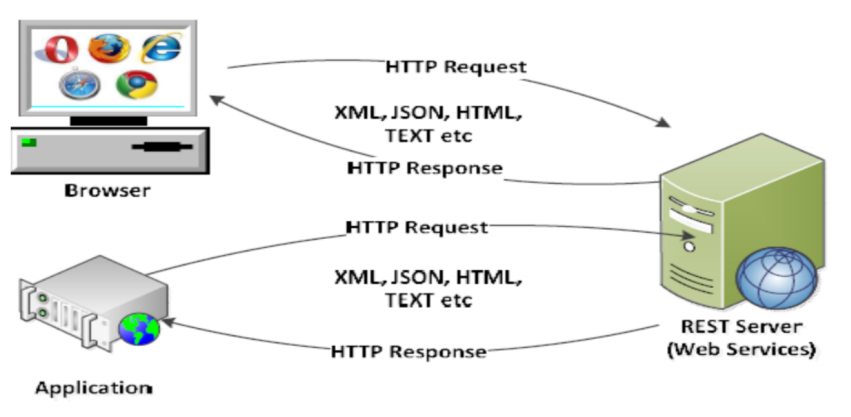
\includegraphics[width=0.9\linewidth]{imagens/rest.png}
	\caption[Exemplo de arquitetura REST]{Exemplo de arquitetura REST \cite{thu2015developing}}
	\label{fig:rest}
\end{figure}

\textbf{RESTful}

Como forma de mensurar a qualidade dos sistemas REST, \citeonline{richardson2008justice} definiu um modelo que possibilita a avaliação do nível de maturidade da arquitetura implementada. Esse modelo é dividido em quatro níveis, sendo que o autor define o último nível como a "glória dos sistemas REST". A organização desses níveis pode ser vista na figura \ref{fig:restNiveis}:

\begin{figure}[H]
	\centering
	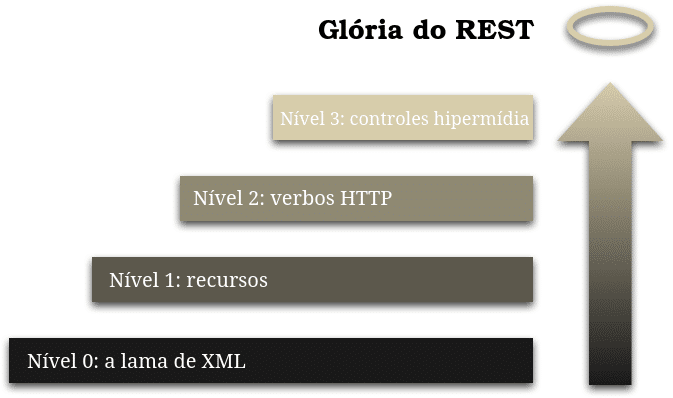
\includegraphics[width=0.7\linewidth]{imagens/restNiveis.png}
	\caption[Níveis da arquitetura REST]{Níveis da arquitetura REST \cite{fowler2010richardson} (adaptado)}
	\label{fig:restNiveis}
\end{figure}

Segundo \citeonline{richardson2008justice} os níveis da arquitetura podem ser definidos da seguinte forma:

\begin{itemize}
    \item \textbf{Nível 0:} Como ponto de partida do modelo, têm-se a utilização do protocolo HTTP para transporte das solicitações, sem utilização de qualquer mecanismos da web. Neste modo, o uso do HTTP apresenta-se normalmente a partir de um mecanismo de encapsulamento, onde é feita uma requisição para determinado endereço que irá realizar a chamada de algum método do sistema, como apresentado na figura \ref{fig:nivel0}. Neste nível, não existe preocupação em relação aos status e retorno das requisições realizadas.
    
    \begin{figure}[H]
    	\centering
    	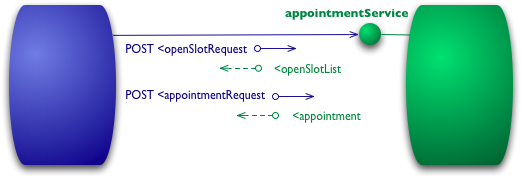
\includegraphics[width=0.7\linewidth]{imagens/level0.png}
    	\caption[Nível 0 no modelo de maturidade]{Nível 0 no modelo de maturidade \cite{fowler2010richardson}}
	    \label{fig:nivel0}
    \end{figure}
    
    \item \textbf{Nível 1:} Para atingir esse nível de maturidade, é necessário a introdução de recursos no sistema. Então, levando em conta a figura \ref{fig:nivel0}, ao invés da chamada a um método do sistema, será realizada a requisição de um recurso, como apresentado na figura \ref{fig:nivel1}:
    
    \begin{figure}[H]
    	\centering
    	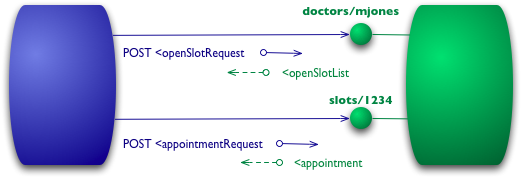
\includegraphics[width=0.7\linewidth]{imagens/level1.png}
    	\caption[Nível 1 no modelo de maturidade]{Nível 1 no modelo de maturidade \cite{fowler2010richardson}}
	    \label{fig:nivel1}
    \end{figure}
    
    \item \textbf{Nível 2:} Neste nível, têm-se a preocupação da correta utilização dos verbos HTTP e seus respectivos status, o que acaba tornando as operações mais semânticas e legíveis para seus utilizadores. Na figura \ref{fig:nivel2}, podemos ver as alterações em relação ao nível 1:
    
    \begin{figure}[H]
    	\centering
    	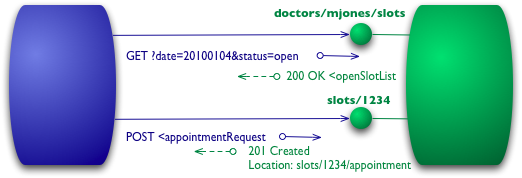
\includegraphics[width=0.7\linewidth]{imagens/level2.png}
    	\caption[Nível 2 no modelo de maturidade]{Nível 2 no modelo de maturidade \cite{fowler2010richardson}}
	    \label{fig:nivel2}
    \end{figure}
    
    \item \textbf{Nível 3:} No nível final de maturidade, é vista a introdução do conceito de HATEOAS (\textit{Hypertext As The Engine Of Application State}). Esse recurso possibilita uma visão dos relacionamentos e das ações possíveis a partir de determinado recurso no sistema. Para realização dessa técnica, são utilizados \textit{hyperlinks} que serão enviados juntamente com a resposta do servidor, explicitando os recursos e ações vinculados ao recurso solicitado. Na figura \ref{fig:nivel3}, temos uma visão desse nível:
    
    \begin{figure}[H]
    	\centering
    	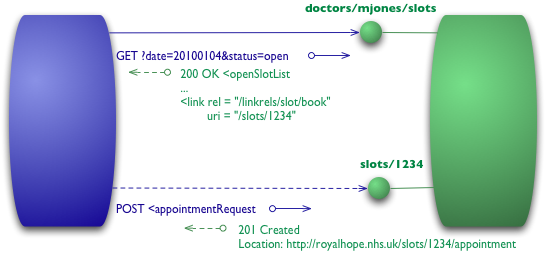
\includegraphics[width=0.7\linewidth]{imagens/level3.png}
    	\caption[Nível 3 no modelo de maturidade]{Nível 3 no modelo de maturidade \cite{fowler2010richardson}}
	    \label{fig:nivel3}
    \end{figure}
\end{itemize}

A utilização do modelo RESTful permite a criação de aplicações distribuídas escaláveis, além de adicionar poderosas descrições e interoperabilidade entre os dados semânticos fornecidos pelo sistema \cite{restfulPerformance}.